\documentclass{report}

\usepackage{blindtext}

\usepackage{amsmath}

\usepackage{graphicx}
\graphicspath{{images/}{../images/}}

\usepackage[utf8]{inputenc}

\usepackage[nottoc]{tocbibind}
\usepackage{natbib}

\usepackage{listings}

\usepackage{multirow}

\usepackage{textcomp}
\usepackage{pgfplots}

\usepackage{algorithm}
\usepackage{algpseudocode}

\usepackage{chngcntr}
\counterwithout{figure}{chapter}
\counterwithout{equation}{chapter}

\pgfplotsset{width=10cm,compat=1.9}

\setcounter{secnumdepth}{5}

\usepackage{pgfplotstable}
\usepgfplotslibrary{groupplots}

\usepackage[section]{placeins}

\usepackage{hyperref}

\usepgfplotslibrary{fillbetween}

\usepackage[autostyle]{csquotes}
\usepackage{caption}
\usepackage{subcaption}

\usepackage{xcolor}
\usepackage{varwidth}

\makeatletter
\renewcommand{\ALG@beginalgorithmic}{\small}
\makeatother


\begin{document}

\begin{titlepage}
    \centering
    
\includegraphics[scale=0.35]{logo.jpg} \par\vspace{1cm}
    {\scshape\LARGE Umeå University \par}
    {\scshape\Large Department of Computing Science\par}
    \vspace{1cm}
    {\scshape\Large Artificial intelligence\par}
    {\scshape\Large Methods and applications\par}
    \vspace{0.5cm}
    {\scshape\large 5DV181\par}
    \vspace{1.5cm}
    {\huge\bfseries Map maker\par}
    \vspace{2cm}
    {\Large\itshape Thomas Ranvier \hspace{1.5cm} Valentin Lecompte \par}
    {\Large\itshape ens18trr \hspace{3.5cm} ens18vle\par}
    \vfill 
    {\large supervised by\par}
    Ola \textsc{Ringdahl}
    \\
    Juan \textsc{Carlos Nieves Sanchez}
    \vfill 
    {\large January 10, 2019\par}
\end{titlepage}


\chapter*{Abstract}
\blindtext


\tableofcontents

\chapter{How to use our program}
\section{Code structure}

Our program is divided in three main modules, the mapping module, the planning module and the controller module.
The role of the first one is to build the map of the environment of the robot using the echoes of the lasers.
The role of the second one is to plan the goal of the robot and the path that the robot must follow in order to explore the world.
The role of the controller module is to make the robot move towards its goal while avoiding the obstacles in its way.

To communicate with the MRDS server we created a class named 'Robot', it is used as an interface to send and receive informations to and from the MRDS server easily.
The received informations are directly adapted to our needs and stored using our 'Position' and 'Laser' datastructures in this class.

\section{How to run our program}

For this assignment we used Python 3 as programming language, to run the program you can use the following syntax:

\begin{lstlisting}[language=bash]
> python3 main.py
\end{lstlisting}


Our program is divided in two main modules, the mapping module and the planning module.
The role of the first one is to build the map of the environment of the robot using the echoes of the lasers.
The role of the second one is to plan the path that the robot must follow in order to explore the world.

To communicate with the MRDS server we created a class named 'Robot', it is used as an interface to send and receive informations to and from the MRDS server easily.
The received informations are directly adapted to our needs and stored using our 'Position' and 'Laser' datastructures in this class.

\chapter{Mapping}
The first point on which we worked was to find a way of building a map of the environment of the robot using the lasers echoes.

To do so we created a class 'Map' that contains a grid of values between $0$ and $1$.
Those values represent probability that there is an obstacle on that cell.
All the values are initialized to $0.5$ which is the average value between $0$ and $1$ since we do not know if there is an obstacle or not at that place.

To update this grid we created a class 'Cartographer' that uses the echoes of the lasers.
For each laser echoe we compute the distance between the robot cell and the cell hit by the laser in the grid.
Then we use the 'Bresenham' algorithm to update all the cells in between the two above.
For all those cells we compute an increment that is added or subtracted to them using the following procedure:

\begin{enumerate}
    \item First we compute an increment value in regard of the value of the cell, the values for max and min increments are respectfully 0.15 and 0.015:
        \begin{itemize}
            \item[$-$] If the cell is a hit cell, meaning that it is the cell where the laser echoed back:
            $$
                inc\_iro\_certainty = min\_increment\texttt{ if }is\_empty(cell)\texttt{ else }max\_increment
            $$
            \item[$-$] If the cell is not a hit cell:
            $$
                inc\_iro\_certainty = min\_increment\texttt{ if }is\_obstacle(cell)\texttt{ else }max\_increment
            $$
        \end{itemize}
    \item Then we compute an increment factor in regard of the distance between the robot and the cell to update:
        $$
        inc\_factor\_iro\_dist = 1 - abs(distance / max\_lasers\_distance)
        $$
    \item The final increment is computed by multiplying the factor with the defined increment:
        $$
        final\_increment = inc\_iro\_certainty \cdot inc\_factor\_iro\_dist
        $$
    \item The final increment is added to the cell if the cell corresponds to the cell hit by the laser and that the distance of the echoe is below the maximum laser distance.
        Otherwise it is subtracted.
\end{enumerate}

With this method when a cell is qualified as obstacle it will be 10 times harder to decrement its value than to increment it and reversely.
That makes the map more consistent because even when the robot hits something which make it shake or turns very fast we will not have false values in our grid.
The distance factor is useful because it will make the cells near the robot update more easily than the cells far away, since the further away the cell is from the robot the less precise the laser information is.

This is the factory map built moving the robot by hand using the cartographer described above.

\FloatBarrier
\begin{figure}
    \centering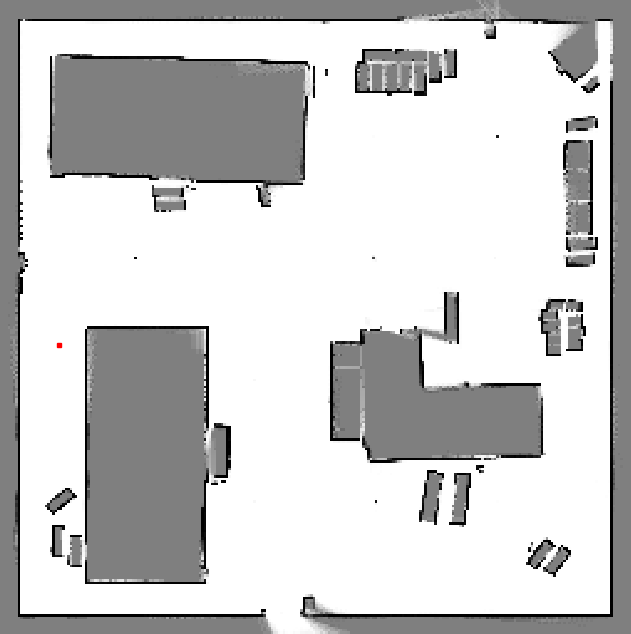
\includegraphics[width=\textwidth]{explored_map_by_hand.png}
    \label{fig:explored_map_by_hand}
    \caption{Explored map by hand}
\end{figure}
\FloatBarrier

The mapping module also contains the 'ShowMap' class which is used to display the built map.


\chapter{Planning}
The planning module is divided in three different parts.

\begin{enumerate}
    \item The first thing to do is to find a goal point, that goal point must be chosen in a way that will make the robot explore unknown parts of the environment.
    \item Then we have to build a path for the robot to follow between the actual position of the robot and the target.
    \item The final thing to do is to use a path tracking algorithm that will make the robot follow the built path.
\end{enumerate}

\section{Find a goal point}

In order to find a goal point we have to detect an unexplored zone that we can access to, to do so we used an approach based on frontier detection.
A frontier is a region on the border between an explored zone and an unexplored zone.
Then the first thing to do in order to determine the next goal point is to detect the frontiers.

\subsection{Detect the frontiers}

To detect the frontiers we go through all the unexplored cells of the grid and if that cell has an explored empty cell in its Von Neumann neighbourhood we know it is part of a frontier.
The Von Neumann neighbourhood is composed of the four adjacent cells around a cell.
Once we went through the whole grid we have a list of all the cells that are on a frontier, the next step is to divide them into several regions.

To divide the frontiers in regions we go through the previously built list, each time we put a cell in its region we delete it from the initial list.
For each cell we go through its Moore neighbourhood (The entire 8 cells neighbourhood).
If one of its neighbour is in the initial list we recursively call the same function.

This is the pseudocode of the 'get\_divided\_frontiers' function:

\FloatBarrier
\begin{algorithm}
    \caption{get divided frontiers}
    \label{get divided frontiers}
    \begin{algorithmic}[1]
        \Procedure{get\_frontiers}{$map$}
            \State $frontiers$ is an empty array
            \For{$cell$ \textbf{in} $map$}
                \If{$is\_unknown(cell)$}
                    \For{$neighbour$ \textbf{in} $von\_neumann\_neighbourhood(cell)$}
                        \If{$neighbour$ \textbf{not in} $frontiers$ \textbf{and} $is\_empty(neighbour)$}
                            \State $frontiers.append(neighbour)$
                        \EndIf
                    \EndFor
                \EndIf
            \EndFor
            \State \textbf{return} $frontiers$
        \EndProcedure
        \Procedure{build\_frontiers}{$frontiers,$ $current\_frontier,$ $cell$}
            \State $neighbours \gets moore\_neighbourhood(cell)$
            \For{$neighbour$ \textbf{in} $neighbours$}
                \If{$neighbour$ \textbf{in} $frontiers$}
                    \State $current\_frontier.append(neighbour)$
                    \State $frontiers.remove(neighbour)$
                    \State $build\_frontier(frontiers, current\_frontier, cell)$
                \EndIf
            \EndFor
        \EndProcedure
        \Procedure{get\_divided\_frontiers}{$map$}
            \State $frontiers \gets get\_frontiers$
            \State $divided\_frontiers$ $is$ $an$ $empty$ $array$
            \While{$frontiers$ \textbf{is not} $empty$}
                \State $current\_frontier$ $is$ $an$ $empty$ $array$
                \State $cell \gets frontiers.pop(0)$
                \State $current\_frontier.append(cell)$
                \State $build\_frontier(frontiers, current\_frontier, cell)$
                \State $divided\_frontiers.append(current\_frontier)$
            \EndWhile
            \State \textbf{return} $divided\_frontiers$
        \EndProcedure
    \end{algorithmic}
\end{algorithm}
\FloatBarrier

On the following figure we can see an example of the detected frontiers, the black pixels are obstacles, the white ones are empty cells, the red spot is the robot position and the other spots are the regions of frontiers. 
The map is 10 by 10 and there is a different color for each region.

\FloatBarrier
\begin{figure}
    \centering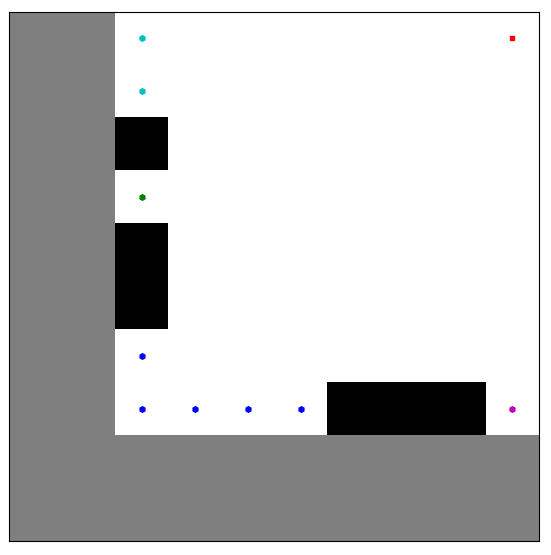
\includegraphics[width=0.5\textwidth]{frontiers.png}
    \label{fig:frontiers}
    \caption{frontiers}
\end{figure}
\FloatBarrier

\section{Build the path}

\section{Follow the path}



\chapter*{Conclusion}
\addcontentsline{toc}{chapter}{Conclusion}
\blindtext


\listofalgorithms
\addcontentsline{toc}{chapter}{List of algorithms}

\end{document}
